\documentclass{standalone}
\usepackage{tikz}
\usetikzlibrary{trees}

\begin{document}

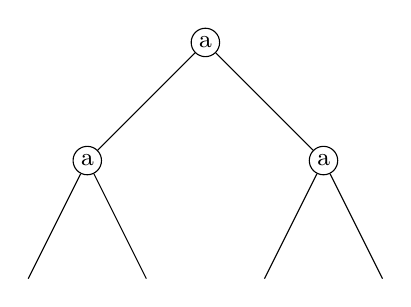
\begin{tikzpicture}[
  level distance = 15mm,
  level 1/.style = {sibling distance = 30mm},
  level 2/.style = {sibling distance = 15mm},
  inner node/.style = {circle, draw, inner sep=1.5pt, font=\small},
  edge from parent/.style = {draw, -},
  leaf/.style = {coordinate} % Leaves are coordinates (invisible points)
]

% Root node
\node[inner node] {a}
  % First child (inner node)
  child { node[inner node] {a}
    % Children of first inner node (leaves)
    child { node[leaf] (l1) {} }
    child { node[leaf] (l2) {} }
  }
  % Second child (inner node)
  child { node[inner node] {a}
    % Children of second inner node (leaves)
    child { node[leaf] (l3) {} }
    child { node[leaf] (l4) {} }
  };

% Optional: Add text annotations for leaves (if needed)
% \node[below=2mm of l1, font=\tiny] {c};
% \node[below=2mm of l2, font=\tiny] {c};
% \node[below=2mm of l3, font=\tiny] {c};
% \node[below=2mm of l4, font=\tiny] {c};

\end{tikzpicture}

\end{document}